
\section{Empirical Evaluation}\fnremark{Start this section with the experimental rationale... what
  hypotheses are we trying to evaluate in this section?}
  
In this section we compare the performance of non-homogeneous solutions with homogeneous solutions. Our hypothesis is that an aggregate plan formed from a set of shorter planning steps, will converge on the optimum plan as the amount of look ahead at each step is increased. We then exploit the non-homogeneity of the QTM to vary \DT[] over the planning period and sample with less resolution as we approach the planning horizon. Compared with a homogenous step with the same number of samples points, each non-homogenous planning step will have a greater look ahead, but with decreasing resolution. Reducing the resolution with look ahead seems reasonable as the accuracy of the plan will also reduce over time when compared with the actual state of the network that eventuates. \fnremark{Add a planning horizon to the planning figure}

\subsection{Networks}

To demonstrate the scalability of the QTM, we evalute three networks of increasing complexity
in the comparison. The first consists of an avenue crossed by three 
side streets at controlled intersections, as shown in \cref{fig:network1}. The second introduces a second
parallel avenue to form a gridded network with a total of three controlled
intersections, as shown in \cref{fig:network2}. And the third is a more complex
grid network with 9 controlled intersections between six avenues, with a seventh avenue running through at a diagonal as shown in \cref{fig:network3}.

The traversal time of each queue in all three networks is set at 9s 
between intersections (a distance of about 100m with a free flow speed of
50km/h). The maximum capacity of each queue not leading in from the boundary of the network
is set at 60 cars. For queues leading in from the boundary, the capacity is increased sufficiently
to buffer any spill back from the stop line and prevent interruption of the input demand profile .
Flows are defined from the head of each queue into the
tail of the next. There is no turning traffic, and in all cases the
maximum flow rate between queues is set at 5 cars per second. Each intersection in networks 1 and 2 has
two phases - North-South (NS) and East-West (EW). In network 3, lights 2, 4 and 6 have an
additional Northeast-Southwest phase to control the diagonal avenue. For networks 1 and 2 for all phases \PTMIN{}{} is 1s
and \PTMAX{}{} is 3s, and for all intersections \CTMIN{}{} is 2s and \CTMAX{}{} is 6s. In network 3 for all phases \PTMIN{}{} is 1s
and \PTMAX{}{} is 6s, and for all intersections \CTMIN{}{} is 2s and \CTMAX{}{} is 12s except for lights 2, 4 and 6 which have a \CTMIN{}{} of 3s and \CTMAX{}{} of 18s.


\subsection{Experimental Methodology}
For each network a background level of inflow is first established and left to run for 55s to allow the solver to settle on a stable policy. Then a spike in demand is introduced to some of the input queues for 15s to trigger a policy change, with the expectation that plans generated with longer look ahead will produce a more coordinated global policy change. The demand is then returned to the background level for another 15s before being reduced to zero, and finally sufficient time is given to allow the network to clear of traffic. By clearing the network we can easily measure the total travel time for all the traffic as the area between the cumulative arrival and departure curves measured at the boundaries of the network. The details of the demand profile per queue are given in \cref{tab:network_demand}.

For both the homogeneous and non-homogeneous test points,
we start by generating a plan for a longer horizon than needed (the look ahead). We then keep the
first part of this plan where the accuracy is highest and discard the
rest. We call the long term plan a major frame, and the first part of the major frame that we retain, a minor frame. While the minor frame
plan is being executed on the network, we generate another major frame starting from the end of the current minor frame and
repeat (see \cref{fig:multiplan}). At each test point we use a minor frame of 10s and increase major frame sizes across the test points from 20 upwards. We generated plans for all three networks with both a homogeneous $\DT[]$ of 0.25s
and a non-homogeneous $\DT[]$ ranging from fixed 0.25s increments
during the minor frame and then increasing linearly until reaching 1s at
the end of the major frame. For reference we also performed a full optimal solve using a
fixed $\DT[]$ of 0.25s. Once we have generated a set of minor
frames, we aggregated them into a single plan and simulate the flow
of through the network using the QTM LP formulation with a fixed $\DT[]$ of 0.25s.
To solve each major frame we use Gurobi with 12 threads on an AMD Opteron 4334 Processor with 12 cores running at 3.4 GHz. We limit MIP gap accuracy to 0.1\% and, while we can solve non-homogeneous major frames up to the convergence point in real time, we extend the solve time cap to 3000s for all test points for a fair comparison with the homogeneous test points. At each test point we take the average of five runs of the solver.

\begin{figure*}[t!]
\centering
%  trim={<left> <lower> <right> <upper>}
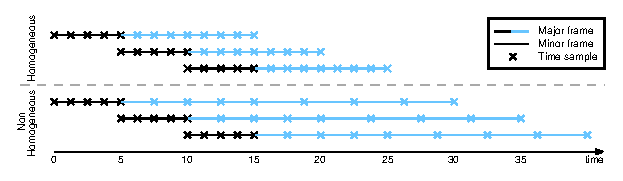
\includegraphics[width=1.0\textwidth]{non_homogeneous_control.eps}
\caption{Multi-step planning}
\label{fig:multiplan}
\end{figure*}


\begin{figure*}[t!]
\centering
%  trim={<left> <lower> <right> <upper>}
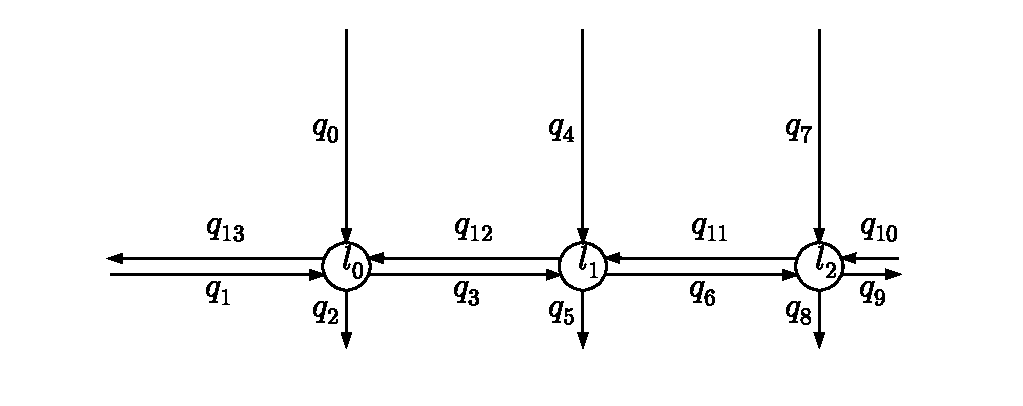
\includegraphics[width=0.75\textwidth]{network_3_lights}
\caption{Network 1}
\label{fig:network1}
\end{figure*}

\begin{figure*}[t!]
\centering
%  trim={<left> <lower> <right> <upper>}
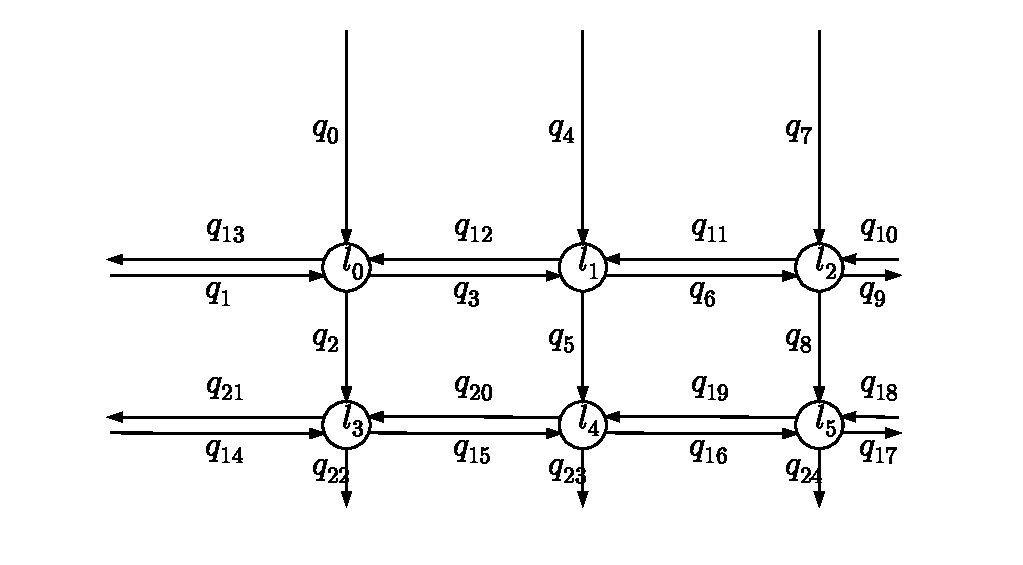
\includegraphics[width=0.75\textwidth]{network_6_lights}
\caption{Network 2}
\label{fig:network2}
\end{figure*}

\begin{figure*}[t!]
\centering
%  trim={<left> <lower> <right> <upper>}
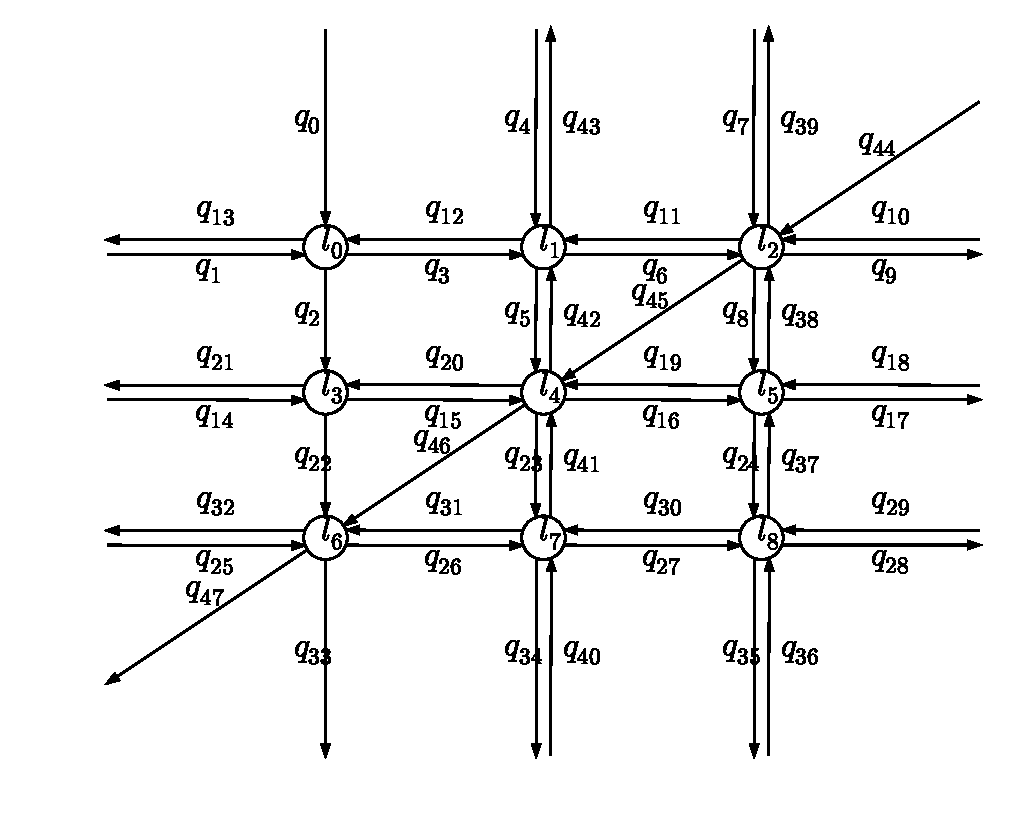
\includegraphics[width=0.75\textwidth]{network_9_lights}
\caption{Network 3}
\label{fig:network3}
\end{figure*}


\begin{table}[h]
\caption{Network Demand Profiles (vehicles per second)}
\label{tab:network_demand}
\centering
\begin{tabular}{cccccc}
\toprule
& Inflow Queues & 0 - 55 s & 55 - 70 s & 70 - 85 s & > 85 s\\
\midrule
\multirow{2}{*}{Network 1}&$q_0$ & 1 & 1 & 1 & 0 \\
&$q_4, q_7$ & 4 & 4 & 4 & 0 \\
&$q_1,q_{10}$& 2 & 4 & 2 & 0 \\
\midrule
\multirow{2}{*}{Network 2}&$q_0$ & 1 & 1 & 1 & 0 \\
&$q_4,q_7,q_{14}$& 4 & 4 & 4 & 0 \\
&$q_1, q_{10},q_{18}$ & 2 & 4 & 2 & 0 \\
\midrule
\multirow{2}{*}{Network 3}&$q_0$ & 1 & 1 & 1 & 0 \\
&$q_4,q_7,q_{14},q_{25},$& 4 & 4 & 4 & 0 \\
&$q_1, q_{10},q_{18},q_{29},q_{36},q_{40},q_{44}$ & 2 & 4 & 2 & 0 \\
\bottomrule\\
\end{tabular}
\end{table}




%\begin{table}[h]
%\caption{Network 3 traffic parameters}
%\label{tab:net3wave}
%\centering
%\begin{tabular}{cccccc}
%\toprule
%Queue & Background & End & Wave & Start &End\\ 
%\midrule
%$q_0$ & 1 & 85 & 1 & 55 & 70\\
%$q_1$ & 2 & 85 & 4 & 55 & 70\\
%$q_4$ & 4 & 85 & 4 & 55 & 70\\
%$q_7$ & 4 & 85 & 4 & 55 & 70\\
%$q_{10}$ & 2 & 85 & 4 & 55 & 70\\
%$q_{14}$ & 4 & 85 & 4 & 55 & 70\\
%$q_{18}$ & 2 & 85 & 4 & 55 & 70\\
%$q_{25}$ & 4 & 85 & 4 & 55 & 70\\
%$q_{29}$ & 2 & 85 & 4 & 55 & 70\\
%$q_{36}$ & 2 & 85 & 4 & 55 & 70\\
%$q_{40}$ & 2 & 85 & 4 & 55 & 70\\
%$q_{44}$ & 2 & 85 & 4 & 55 & 70\\
%\bottomrule\\
%\end{tabular}
%\end{table}

\subsection{Results}

We compare the performance of non-homogeneous and homogeneous solutions in two ways: comparing the decrease in total travel time with increasing major frame time, and analysing the distribution of delay in each queue of the network. \cref{subfig:travel_time_3,subfig:travel_time_6,subfig:travel_time_9} show a comparison between the number of time samples used in the major frame vs the \% improvement in total travel time. It can be seen that for all networks, using a non homogeneous $\DT[]$ converges towards the optimum total travel time more quickly than the homogeneous $\DT[]$. 

\cref{subfig:delay_3,subfig:delay_6,subfig:delay_9} show a comparison of distribution of delay across the network. This gives us an indication of the quality of the solution in terms of the number of vehicles that experience significant delay and if the plan may be starving some parts of the network.  The box plots show three comparisons: at the point where the non-homogeneous $\DT[]$ first converges on the optimum solution, where the homogeneous $\DT[]$ first converges on the optimum solution, and the optimum solution. With all three networks the quality of the solutions improves or stays the same using a non-homogeneous $\DT[]$ compared to a homogeneous $\DT[]$.
Finally, \cref{fig:cumu} shows the cumulative arrival and departure curves and the how delay evolves over time for $q_1$ of network 2. \cref{subfig:cumu1} shows the comparison at the point where the non-homogeneous $\DT[]$ first converges and shows that with the longer major frame time of the non-homogeneous $\DT[]$, the solver is able to find a co-ordinated signal policy along the avenue to dissipate the extra traffic that arrives at the 55s point, while the homogeneous $\DT[]$ with its shorter major frame fails to find a coordinated policy along the avenue. Once the homogeneous $\DT[]$ has converged in \cref{subfig:cumu2}, both solutions are close to the optimum shown in \cref{subfig:cumu3}.

\begin{figure*}[t!]
\centering

%  trim={<left> <lower> <right> <upper>}
\subfigure[]{
\label{subfig:travel_time_3}
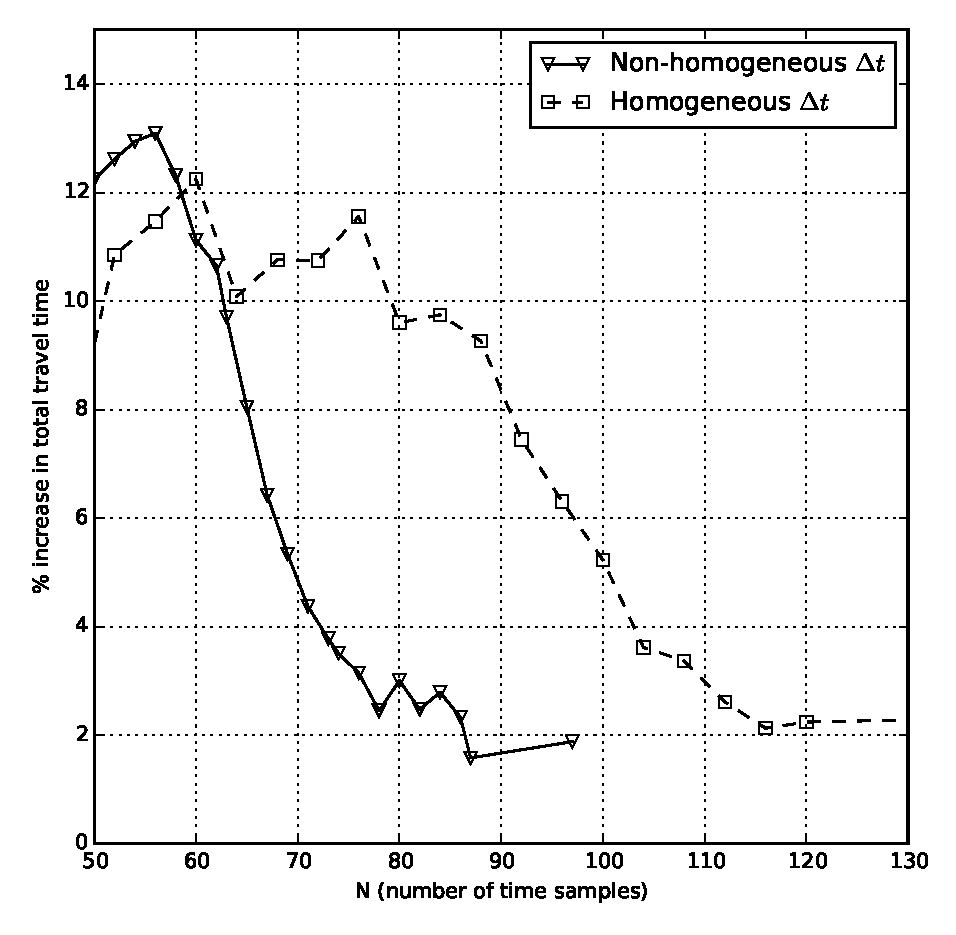
\includegraphics[width=0.4\textwidth]{samples_plot_3_lights}}
\subfigure[]{
\label{subfig:delay_3}
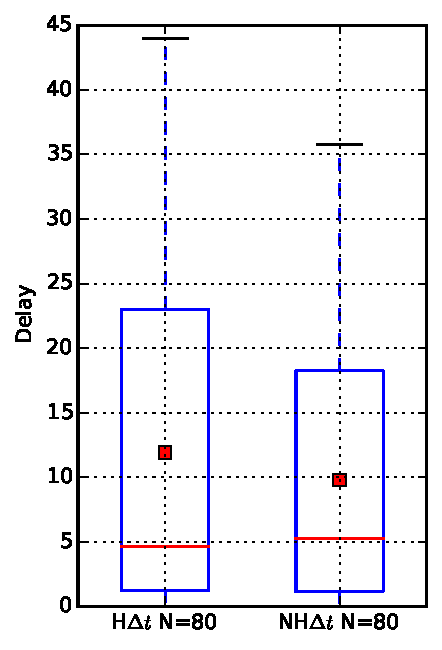
\includegraphics[keepaspectratio,height=0.3\textwidth]{box_plot_early_3l.pdf}
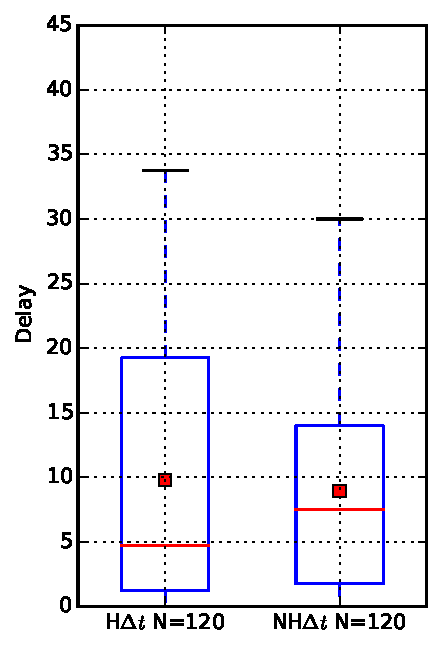
\includegraphics[keepaspectratio,height=0.3\textwidth]{box_plot_converg_3l.pdf}
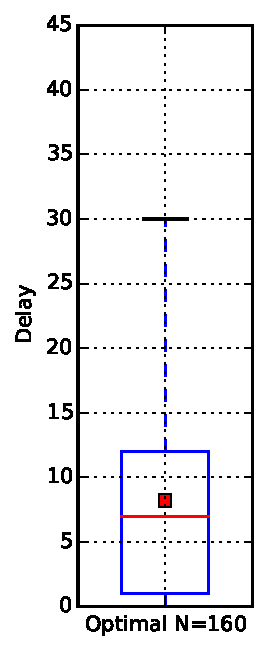
\includegraphics[keepaspectratio,height=0.3\textwidth]{box_plot_final_3l.pdf}}

\subfigure[]{
\label{subfig:travel_time_6}
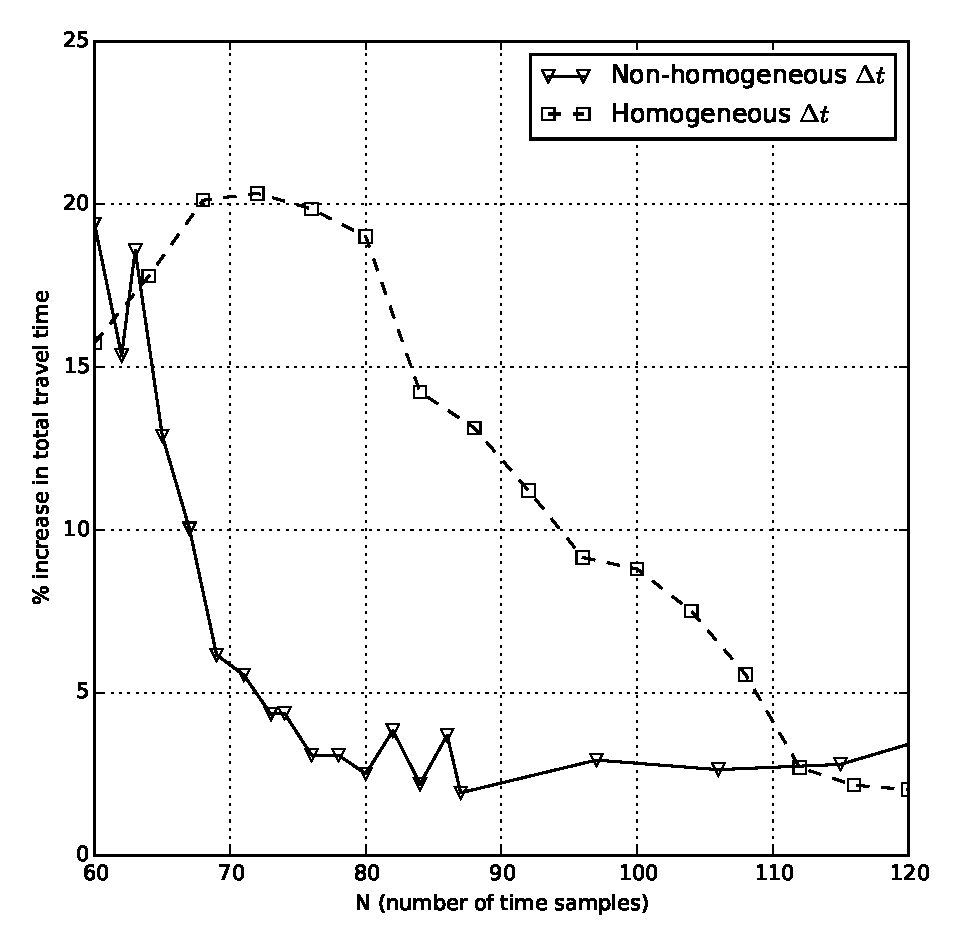
\includegraphics[width=0.4\textwidth]{samples_plot_6_lights}}
\subfigure[]{
\label{subfig:delay_6}
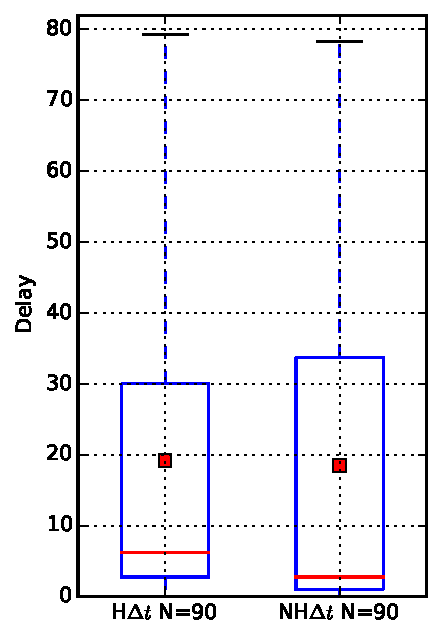
\includegraphics[keepaspectratio,height=0.3\textwidth]{box_plot_early_6l.pdf}
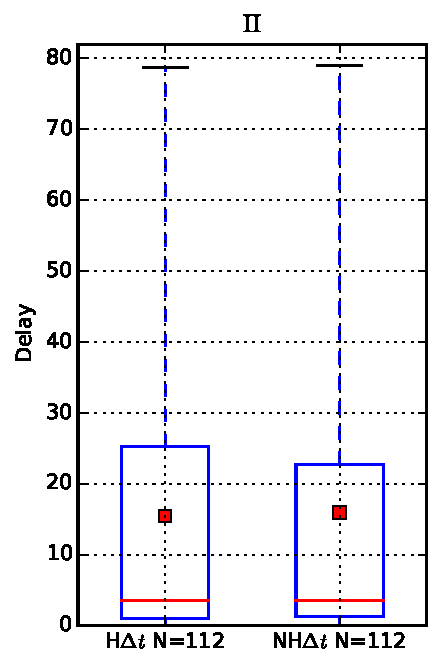
\includegraphics[keepaspectratio,height=0.3\textwidth]{box_plot_converg_6l.pdf}
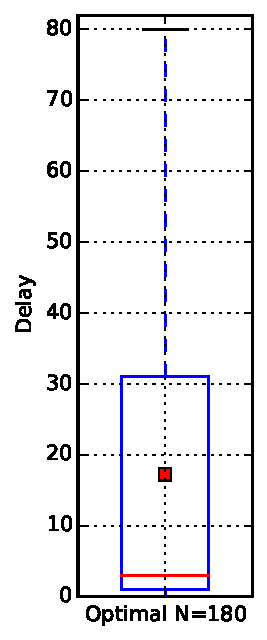
\includegraphics[keepaspectratio,height=0.3\textwidth]{box_plot_final_6l.pdf}}

\subfigure[]{
\label{subfig:travel_time_9}
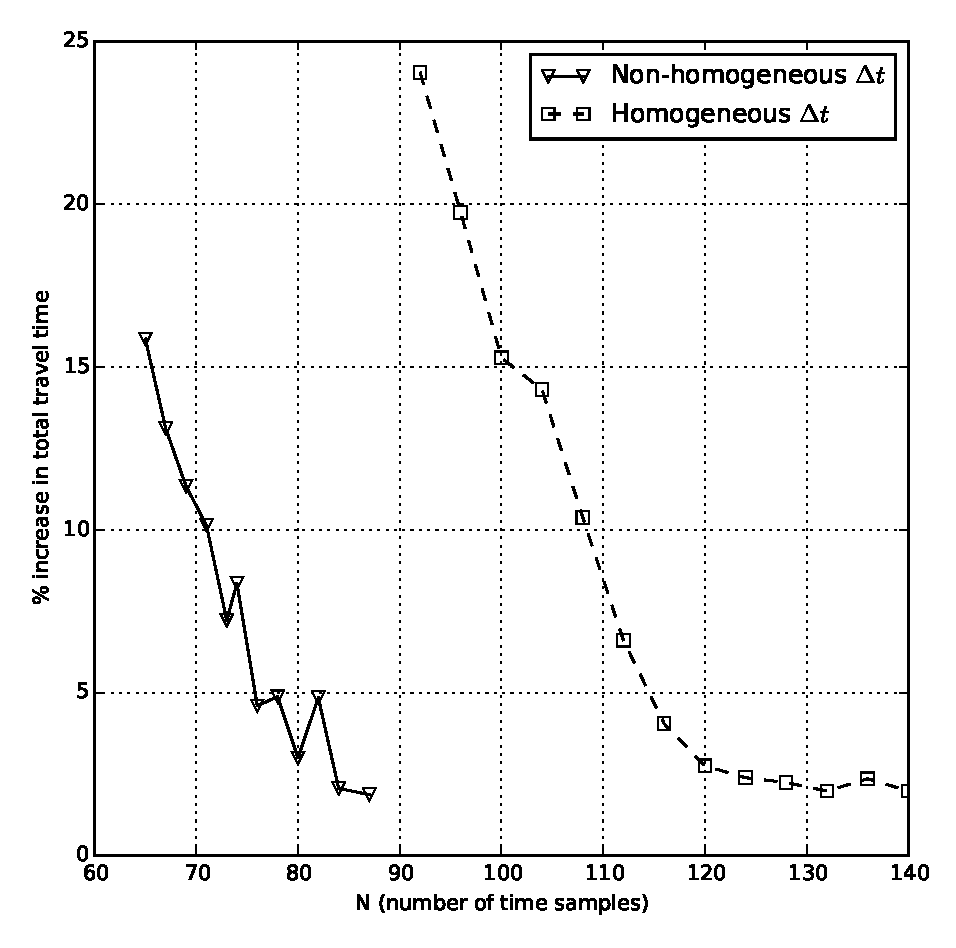
\includegraphics[width=0.4\textwidth]{samples_plot_9_lights}}
\subfigure[]{
\label{subfig:delay_9}
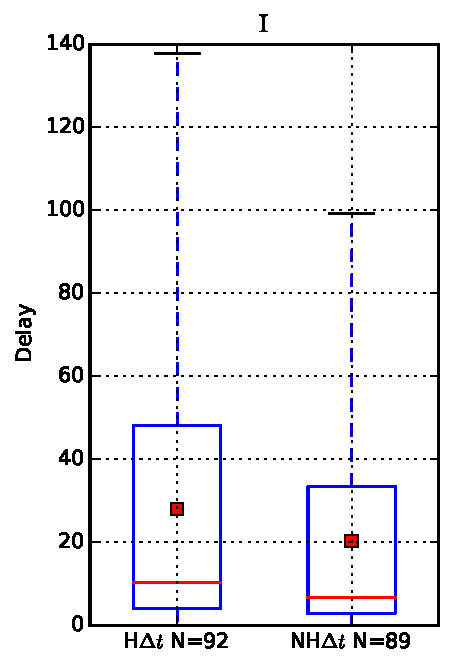
\includegraphics[keepaspectratio,height=0.3\textwidth]{box_plot_early_9l.pdf}
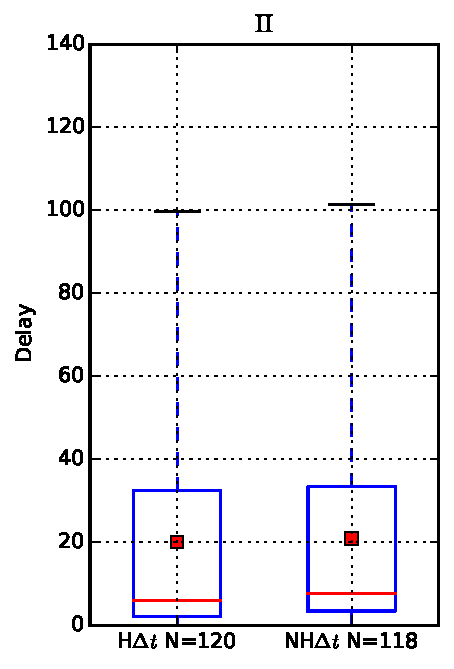
\includegraphics[keepaspectratio,height=0.3\textwidth]{box_plot_converg_9l.pdf}
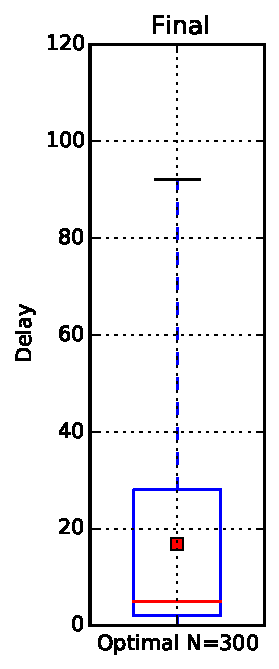
\includegraphics[keepaspectratio,height=0.3\textwidth]{box_plot_final_9l.pdf}}
\caption{Results for the three networks showing the comparitive \% increase in total travel time for the network between using a homogeneous $\DT[]$ and a non-homogeneous $\DT[]$, and the distribution of delay time at the convergence point of non-homogeneous $\DT[]$, the convergence point of homogeneous $\DT[]$ and for the fully solved optimal solution. (a) and (b) 3 light avenue, (c) and (d) 6 light grid, and (e) and (f) 9 light grid,}
\label{fig:results}
\end{figure*}

\begin{figure*}[t!]
\centering

%  trim={<left> <lower> <right> <upper>}
\subfigure[]{
\label{subfig:cumu1}
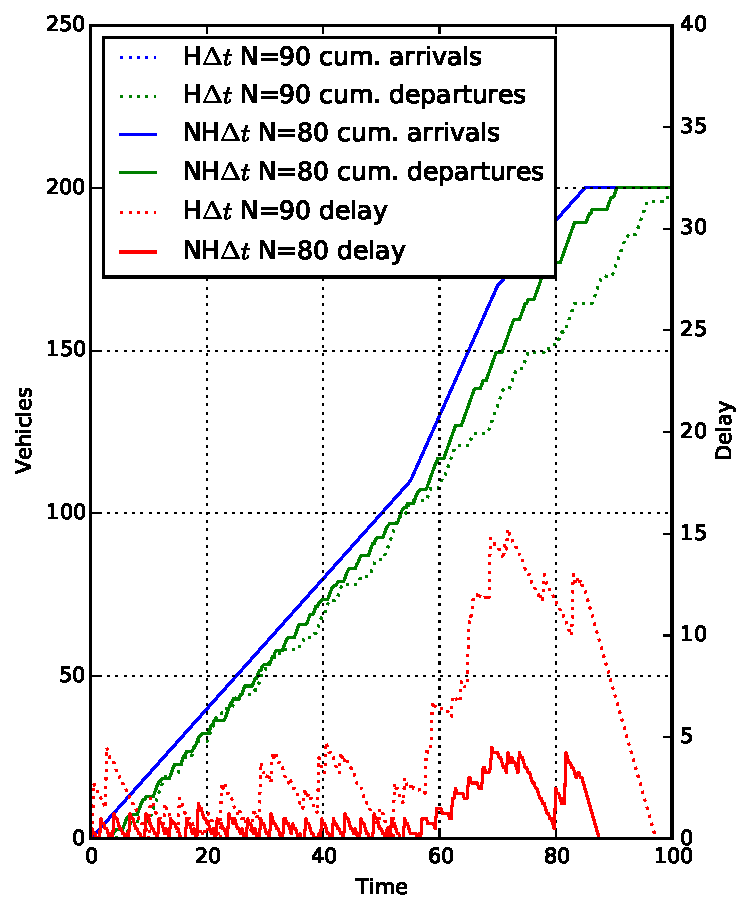
\includegraphics[width=0.32\textwidth]{cum_plot_early_6l.pdf}}
\subfigure[]{
\label{subfig:cumu2}
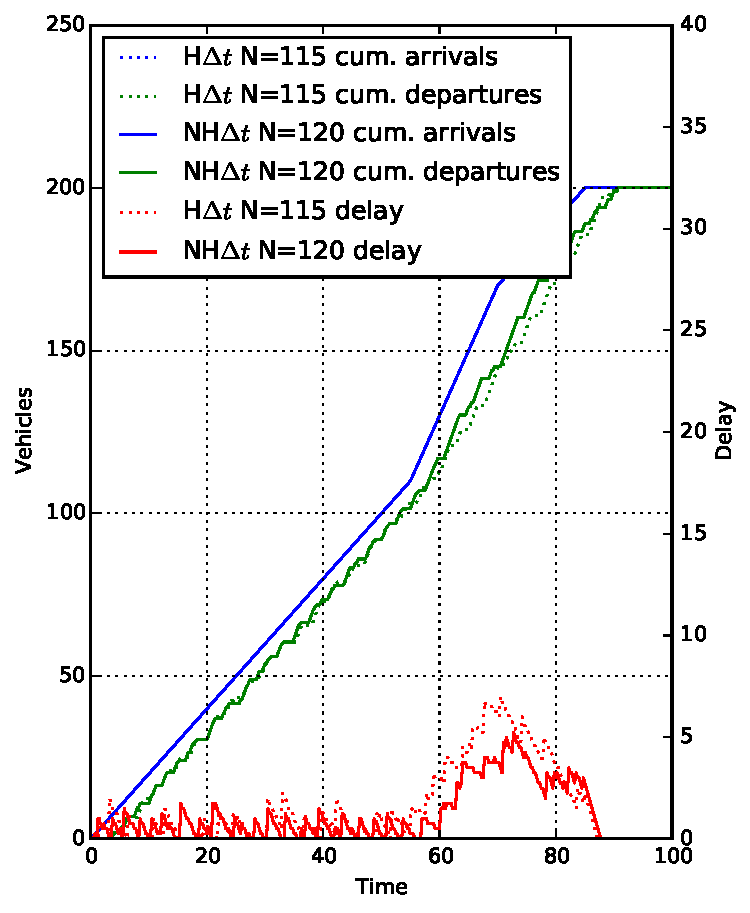
\includegraphics[width=0.32\textwidth]{cum_plot_converg_6l.pdf}}
\subfigure[]{
\label{subfig:cumu3}
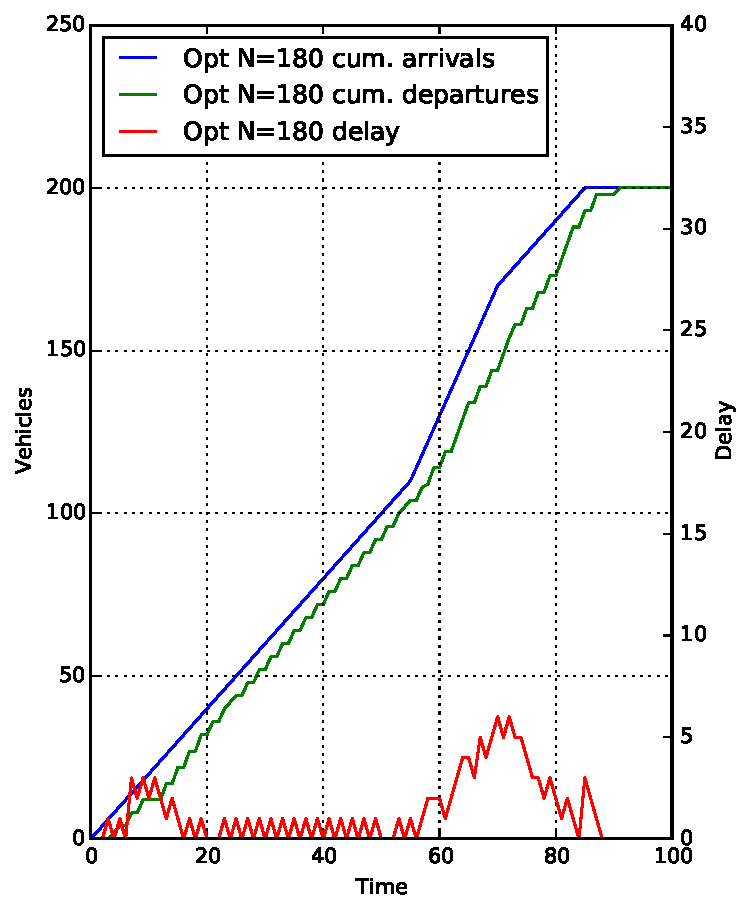
\includegraphics[width=0.32\textwidth]{cum_plot_final_6l.pdf}}
%\includegraphics[width=0.25\textwidth,trim={3cm 1.5cm 3cm 2.3cm},clip]{Satellite_Augmentation/test_17.eps}}
\caption{Cumulative arrival and departure curves and delay for queue 1 in the 6 light grid. (a) at the convergence point of the non-homogeneous $\DT[]$ it is near to the optimum solution while homogeneous $\DT[]$ lags behind (b) at the convergence point of homogeneous $\DT[]$ both are near optimum, and (c) the fully solved optimal solution}
\label{fig:cumu}
\end{figure*}

